\documentclass[12pt, a4paper, oneside]{book}
\usepackage[utf8]{inputenc}
\usepackage[spanish]{babel}
\usepackage{amsmath}
\usepackage{amsfonts}
\usepackage{amssymb}
%\usepackage{makeidx}
\usepackage{graphicx}
\usepackage{csquotes}
\usepackage{tikz}
%\usepackage{lmodern}
%\usepackage{kpfonts}
\usepackage[left=2cm,right=2cm,top=2cm,bottom=2cm]{geometry}
\usepackage{bm}
%\usepackage{cite}
\usepackage[
backend = biber,
bibstyle = apa,
citestyle = numeric, 
sorting = none
]{biblatex}
\usepackage{hyperref}
\usepackage{cleveref}
%\usepackage{autonum}
%\usepackage{comment}
\usepackage{braket}
\usepackage{amsthm}
\usepackage{csquotes}
\usepackage{physics}
\usepackage{fancyhdr}
\usepackage{newtxtext}
\usepackage{newtxmath}
\usepackage{subcaption}
\usepackage[bottom]{footmisc}
\usepackage{fancyhdr}

\graphicspath{{FIGURAS/}}
\addbibresource{falso_vacio.bib}

\usetikzlibrary{babel}

%\numberwithin{equation}{section}

\DeclareFieldFormat{labelnumberwidth}{\mkbibbrackets{#1}}

\defbibenvironment{bibliography}
  {\list
     {\printtext[labelnumberwidth]{%
      \printfield{labelprefix}%
      \printfield{labelnumber}}}
     {\setlength{\labelwidth}{\labelnumberwidth}%
      \setlength{\leftmargin}{\labelwidth}%
      \setlength{\labelsep}{\biblabelsep}%
      \addtolength{\leftmargin}{\labelsep}%
      \setlength{\itemsep}{\bibitemsep}%
      \setlength{\parsep}{\bibparsep}}%
      \renewcommand*{\makelabel}[1]{\hss##1}}
  {\endlist}
  {\item}

\linespread{1.6}

\allowdisplaybreaks

\decimalpoint

%\clearpage\null\thispagestyle{empty}

\begin{document}
	
\frontmatter
	
\begin{titlepage}
\begin{center}

\thispagestyle{empty}

\textsc{\LARGE{Universidad Nacional Mayor de San Marcos}} \\
\large{Universidad del Perú, Decana de América} \\ [0.5cm] 
\textsc{\LARGE Facultad de Ciencias Físicas} \\  
\textsc{\Large Escuela Profesional de Física} \\ [1cm]

\includegraphics*[height = 5cm]{unmsm_logo.png} \\ [1cm]

\textsc{\LARGE Trabajo de Investigación} \\ [0.25cm]
\large \text{Para optar por el grado académico de Bachiller en Física} \\ [0.5cm]

\LARGE{\bfseries{Decaimiento del falso vacío en la Mecánica Cuántica y la Teoría Cuántica de Campos}} \\ [0.5cm] 

\textsc{\LARGE Autor} \\ [0.25cm] 
\large{Erwin Renzo Franco Diaz} \\ [0.5cm]

\textsc{\LARGE Asesor} \\ [0.25cm] 
\large{Teófilo Vargas Auccalla} \\ 

\vfill

\large \text{Lima, Perú} \\ [0.25cm]
\large \text{Abril 2021}

\end{center}
\end{titlepage}

\newgeometry{top = 1in, bottom = 1in, right = 1in, left = 1in}

\addcontentsline{toc}{chapter}{Resumen}

\begin{center}
	\thispagestyle{plain}
	\setlength{\parskip}{0pt}
	{\huge{\textsc{Resumen}} \par}
\end{center}

\colorbox{yellow}{añadir descripcion de capitulos}	

\newpage

\addcontentsline{toc}{chapter}{Agradecmientos}

\begin{center}
	\thispagestyle{plain}
	
	\setlength{\parskip}{0pt}
	{\huge{\textsc{Agradecimientos}} \par}
\end{center}

\addcontentsline{toc}{chapter}{Índice general}
\tableofcontents

\addcontentsline{toc}{chapter}{Índice de figuras}
\listoffigures

\newpage

\begin{center}
	\thispagestyle{empty}
	\hspace{0pt}
	\vfill
	\textit{Dedicado a}
	\vfill
	\hspace{0pt}
\end{center}

\mainmatter

% Chapter Template

\chapter{Introducción} % Main chapter title

\section{Motivación}

Desde su formulación inicial en la década de 1920, se hizo evidente que la Mecánica Cuántica es una teoría radicalmente distinta al resto de la Física conocida hasta ese entonces. Uno de los ejemplos más sorprendentes de esto es el efecto túnel o tunelamiento. Descubierto inicialmente por George Gamow en 1928 para explicar el decaimiento alfa \cite{gamow1928quantum}, este fenómeno permite a una partícula atravesar una barrera de potencial, a pesar de que no pueda hacerlo clásicamente por no contar con la energía suficiente. 

Una consecuencia importante del efecto túnel es el decaimiento del falso vacío, tema principal a tratar en este trabajo. En este caso, la partícula atraviesa la barrera de potencial a la vez que decae al estado de mínima energía. 

El decaimiento del falso vacío tiene implicaciones importantes tanto en la física de partículas como en la cosmología. 

%$\Gamma$ que establece una escala temporal en la cual podría ocurrir. 

\section{Planteamiento del problema}

\colorbox{yellow}{revisar}
Consideremos un potencial como el de la figura \ref{fig:potencial} que posee dos mínimos distintos, uno mayor que otro. Clásicamente, ambos puntos son estables. Sin embargo, esta no es la situación a nivel cuántico. Debido al efecto túnel, existe la posibilidad de que una partícula que se encuentre inicialmente en $x_+$, atraviese la barrera %reapareciendo por $x_0$                                                            
al estado de menor energía del sistema. Es por esto que a $x_+$ se le denomina como falso vacío y a este proceso como decaimiento del falso vacío.

A lo largo del trabajo tomaremos la figura \ref{fig:potencial} como nuestro potencial de referencia. % al momento de realizar los cálculos. 

\begin{figure}[h!]
	\centering
	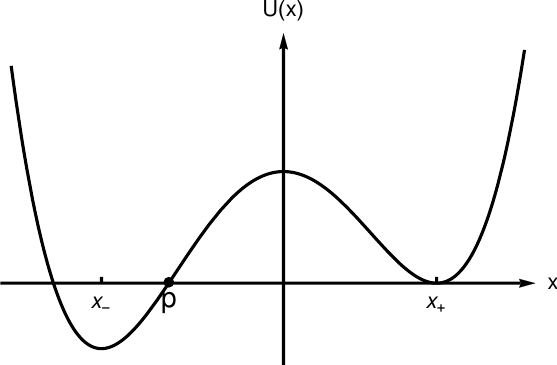
\includegraphics[scale = 0.4]{../FIGURAS/potencial}
	\caption{Potencial con un falso vacío en $x_+$ \cite{Ai:2019dqr}.}
	\label{fig:potencial}
\end{figure}

\section{Objetivo}

El objetivo principal del presente trabajo de investigación es el cálculo de la tasa de decaimiento del falso vacío $\Gamma$ a primer orden en $\hbar$. 
%para el estado metaestable de menor energía
Inicialmente se llevará a cabo en la Mecánica Cuántica haciendo uso de la integral de camino euclideana y la aproximación del punto estacionario siguiendo el formalismo planteado originalmente por Coleman y Callan \cite{coleman1977fate, callan1977fate}. %Primero se estudiará este fenómeno en la Mecánica Cuántica y luego en la Teoría Cuántica de Campos del campo escalar. 
Posteriormente el mismo será extendido a la Teoría Cuántica de Campos del campo escalar donde además se analizará la formación de burbujas de verdadero vacío y su evolución espaciotemporal. 




%\begin{figure}[h]
%	\centering
%	\begin{tikzpicture}[scale = 2]
%	
%	\draw[<->] (-2, 0) -- (2, 0) node[anchor = west] {$x$}; 
%	\draw[<->] (0,-1) -- (0,2) node[anchor = south] {$V(x)$};
%	
%	\draw[line width = 0.5mm, color = blue, domain = -1.5:1.5, smooth] plot(\x, {((\x - 1)^2)*((\x + 1)^2) - 0.2*(\x + 1)});
%	
%	\node[anchor = north] at (-1, 0) (a) {$a$};
%	\draw (-1,-0.05) -- (-1,0.05);
%	
%	\node[anchor = north] at (-1, 0) (a) {$a$};
%	\draw (-1,-0.05) -- (-1,0.05);
%	
%	\node[anchor = southleine] at (1, 0) (b) {$b$};
%	\draw (1,-0.05) -- (1,0.05);
%	\end{tikzpicture}
%	%\caption{Potencial para el estudio numérico del decaimiento del falso vacío. Cuenta con una región de falso (FV) y verdadero vacío (R), separados por una barrera (B) \cite{Masoumi:2015psa}.}
%	%\label{fig:potencial_numerico} 
%\end{figure}








\chapter{Decaimiento del falso vacío en la Mecánica Cuántica} 

%\section{Tunelamiento y aproximación WKB}

%La tasa de decaimiento $\Gamma$ es proporcional al coeficiente de transmisión a través de la barrera $T$. Para un potencial cualquiera es posible obtener $T$ de 
%\begin{equation}\label{eq:gamma}
%	\Gamma = A e^{-B/\hbar} \qty(1 + \order{\hbar})
%\end{equation}

\section{Tasa de decaimiento}

Un estado concentrado en la región del falso vacío no puede ser un autoestado de energía, puesto que estos, al no poseer dependencia temporal, no pueden decaer \cite{andreassen2017precision}. Podríamos expandirlo en una combinación lineal de estos autoestados, pero es más conveniente considerarlo como un estado metaestable cuya energía adquiere una parte imaginaria debido al tunelamiento  \cite{weinberg2012classical, paranjape2017theory}. 

A diferencia de lo que sucede con los autoestados de energía, la evolución temporal del estado metablestable ya no consiste únicamente en la adquisición de una fase \cite{kleinert2009path}
\begin{equation}
e^{iE t/\hbar}\ket{\psi} = e^{i\Re\qty(E) t/\hbar}e^{\Im\qty(E) t/\hbar}\ket{\psi}.
\end{equation}
La parte imaginaria de la energía hace que la probabilidad de que una partícula permanezca en la región del falso vacío, relacionada con la norma del estado metaestable, disminuya exponencialmente en el tiempo 
\begin{equation} \label{eq:prob}
P_{\text{FV}}(t) \propto e^{-\Gamma t/\hbar},
\end{equation}
lo que nos permite definir la tasa de decaimiento $\Gamma$ como
\begin{equation}\label{eq:gammaE}
\Gamma = -2 \, \mathrm{Im}\left(\frac{E}{\hbar}\right).
\end{equation} 
Esta definición considera implícitamente que la parte imaginaria de la energía del estado metaestable es negativa, de tal manera que $\Gamma$ sea positiva. De no ser así, la probabilidad \eqref{eq:prob} crecería, en lugar de decaer, exponencialmente \cite{kleinert2009path}. 

Podemos entender cualitativamente este comportamiento estudiando numéricamente la evolución temporal de una función de onda concentrada inicialmente en la región del falso vacío de un potencial sencillo como el de la figura \ref{fig:potencial_numerico}, y calculando la probabilidad de encontrar a la partícula en esta región luego de un tiempo $t$. Los resultados de la simulación se presentan en la figura \ref{fig:numerico} para distintos anchos de la región de verdadero vacío. Tal como esperábamos, se observa claramente la dependencia lineal de la probabilidad en escala logarítmica con el tiempo. Notamos además que las tres rectas tienen la misma pendiente, lo cual indica que la forma especifica de la parte derecha del potencial no influye de manera significativa en la dinámica del sistema \cite{paranjape2017theory}. 

\begin{figure}[h]
	\centering
	\begin{tikzpicture}
	
	\draw[<->] (6.5, 0) node[anchor = west] {$x$}-- (0,0) -- (0,5) node[anchor = south] {$V(x)$};
	
	\draw[blue, line width = 0.5mm] (0,0.975) -- (0, 4.5);
	\draw[blue, line width = 0.5mm] (-0.025,1) -- (1.025,1);
	\draw[blue, line width = 0.5mm] (1,0.975) -- (1,3.025);
	\draw[blue, line width = 0.5mm] (0.975,3) -- (2.5, 3);
	\draw[blue, line width = 0.5mm] (2.5, 3.025) -- (2.5,-0.025);
	\draw[blue, line width = 0.5mm] (2.475,0) -- (6,0);
	\draw[blue, line width = 0.5mm] (6,0) -- (6, 4.5);
	
	\node at (0.5, 2) (FV) {FV};
	\node at (1.75, 2) (B) {B};
	\node at (4.25, 2) (B) {R};
	
	\end{tikzpicture}
	\caption{Potencial para el estudio numérico del decaimiento del falso vacío. Cuenta con una región de falso (FV) y verdadero (R) vacío, así como una barrera (B).}
	\label{fig:potencial_numerico}
\end{figure}

\begin{figure}
	\centering
	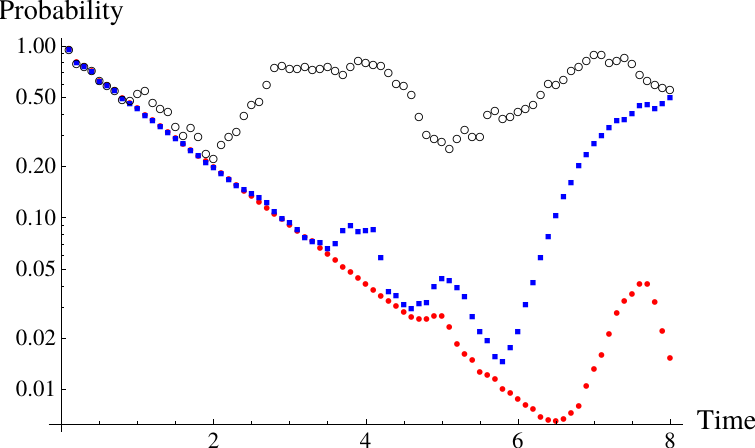
\includegraphics[scale = 0.4]{FIGURAS/numerico}
	\caption{Probabilidad de que una partícula permanezca en la región de falso vacío para distintos anchos de verdadero vacío. El eje vertical está en escala logarítmica \cite{Masoumi:2015psa}.}
	\label{fig:numerico}
\end{figure}

En la misma figura, sin embargo, puede apreciarse que el régimen lineal se mantiene solo durante un cierto intervalo de tiempo. Antes de atravesar la barrera, la función de onda oscila en la región del falso vacío. 
%Esto se puede apreciar más fácilmente en la figura \ref{fig:numericoandreassen}. 
Por otro lado, cuando la función de onda ya atravesó la barrera y se encuentra la región del verdadero vacío, rebota con la pared derecha y empieza a interactuar consigo misma, dando como resultado efectos no lineales \cite{Masoumi:2015psa}. Estos aspectos deben ser tomados en cuenta al momento de definir $\Gamma$ de manera precisa \cite{andreassen2017precision}. 

%\begin{figure}[h]
%	\centering
%	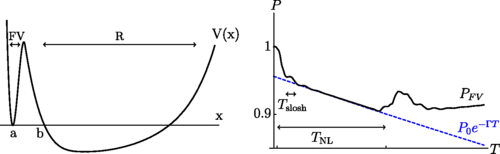
\includegraphics[scale = 0.7]{FIGURAS/numerico_andreassen}
%	\caption{\cite{andreassen2017precision}}
%	\label{fig:numericoandreassen}
%\end{figure}

%Siguiendo el formalismo de Coleman y Callan \cite{coleman1977fate, callan1977fate}, hallaremos una expresión para $\Gamma$ a primer orden en $\hbar$ . Puesto que el tunelamiento es un proceso no perturbativo, se hará uso de la integral de camino euclideana junto con la aproximación de punto estacionario.

\section{Integral de camino euclideana}

%En el capítulo anterior pudimos determinar, analizando el tunelamiento usando la aproximación WKB, que el coeficiente $B$ en \eqref{eq:gamma} corresponde a la acción euclideana del bounce. Para calcular el coeficiente $A$ es necesario usar la integral de camino de Feynman en tiempo euclideano y la aproximación de punto estacionario. 

El objetivo principal de este trabajo es calcular $\Gamma$ a primer orden en $\hbar$ para el estado metaestable de menor energía. Para esto se hará uso de la integral de camino euclideana y la aproximación de punto estacionario siguiendo el formalismo establecido por Coleman y Callan \cite{coleman1977fate, callan1977fate}. 

Consideremos una partícula que inicialmente se encuentra en la posición $x_i$ en un tiempo $t_i$. La amplitud de transición de esta a una posición final $x_f$ en un tiempo $t_f$ está dada por la integral de camino de Feynman \cite{feynman2010quantum}
\begin{equation}\label{eq:amplitud}
\bra{x_f, t_f}\ket{x_i, t_i} = N \int \mathcal{D}x \, e^{iS\qty[x \qty(t)]/\hbar},
\end{equation}
donde $S\qty[x \qty(t)]$ es la acción de la partícula que, de la Mecánica Clásica, sabemos que es está dada por \footnote{A lo largo de todo el trabajo consideraremos que la partícula es de masa unitaria. 
}
\begin{equation}
S\qty[x \qty(t)] = \int \dd{t} \qty[\frac{1}{2} \left(\dv{x}{t}\right)^2 - V\qty(x)] \label{eq:accion}
\end{equation}
y $N$ es una constante de normalización que se debe elegir convenientemente, pero que no será de interés en este trabajo. 
%incluir explicacion de la integral de camino?

Una de las dificultades al momento de querer calcular \eqref{eq:amplitud} se debe al hecho de que está compuesta por una suma de fases complejas oscilatorias, que no necesariamente va a converger. Es por esto que resulta más conveniente trabajar en tiempo imaginario, para lo cual introducimos el tiempo euclideano $\tau$ mediante el cambio de variable
\begin{equation}
	t = -i\tau, \label{tiempo_im}
\end{equation} 
también conocido como rotación de Wick \cite{das2006field}. $\tau$ es un parámetro real. 

Aplicando el cambio de variable \eqref{tiempo_im} en la acción \eqref{eq:accion}, tenemos
\begin{align}
S\qty[x\qty(\tau)] &= \int \dd{\qty(-i\tau)} \qty[ \frac{1}{2} \left(\dv{x}{\qty(-i\tau)}\right)^2 - V(x)] \\
&= -i\int \dd{\tau} \qty[ -\frac{1}{2} \left(\dv{x}{\tau}\right)^2 - V\qty(x)] \\ 
&= i \int \dd{\tau} \qty[ \frac{1}{2}\qty(\dv{x}{\tau})^2 + V(x)] \\
&= iS_E\qty[x\qty(\tau)] \label{eq:S_s_e}
\end{align}
donde hemos definido la acción euclideana $S_E\qty[x\qty(\tau)]$ como 
\begin{equation}\label{eq:eucliaction}
S_E\qty[x\qty(\tau)] \equiv \int \dd{\tau} \qty[ \frac{1}{2}\qty(\dv{x}{\tau})^2 + V(x)].
\end{equation}

Haciendo de igual manera en la ecuación de movimiento
\begin{align}
	\dv[2]{x}{t} &= -\dv{V(x)}{x} \\
	\dv[2]{x}{\qty(-i\tau)} &= -\dv{V(x)}{x} \\
	-\dv[2]{x}{\tau} &= -\dv{V(x)}{x},
\end{align}
obtenemos la correspondiente para  $S_E\qty[x\qty(\tau)]$
\begin{equation}\label{eq:mov_ec}
\dv[2]{x}{\tau} = \dv{V(x)}{x}.
\end{equation}
Podemos entender esta ecuación como la ecuación de movimiento en tiempo real para una partícula moviéndose en el potencial invertido $-V\qty(x)$
\begin{equation}
\dv[2]{x}{\tau} = -\dv{\qty(-V(x))}{x}.
\end{equation}
 
%Integrando la ecuación de movimiento \eqref{eq:mov_ec} respecto a la posición obtenemos la integral de movimiento
%\begin{align}
%	\dv[2]{x}{\tau} - \dv{V(x)}{x} &= 0 \\
%	\dv[2]{x}{\tau} - \dv{V(x)}{x} &= 0
%\end{align} 
Por último, en la energía, 
\begin{align}
	E &= \frac{1}{2} \left(\dv{x}{t}\right)^2 + V\qty(x) \\
	&= \frac{1}{2} \left(\dv{x}{\qty(-i\tau)}\right)^2 + V\qty(x) \\
	&= -\frac{1}{2} \left(\dv{x}{\tau}\right)^2 + V\qty(x) \\
	&= -\mathcal{E}
\end{align}
donde hemos definido la energía euclideana $\mathcal{E}$ como \cite{rubakov2009classical}
\begin{equation}
	\mathcal{E}  \equiv \left(\dv{x}{\tau}\right)^2 - V\qty(x)
\end{equation}

Al reemplazar \eqref{eq:S_s_e} en la integral de camino \eqref{eq:amplitud}, obtenemos la integral de camino euclideana \cite{das2006field}
\begin{equation}\label{eq:amplitud_euc}
I = \bra{x_f}e^{-HT/\hbar}\ket{x_i} = N \int \mathcal{D}x \, e^{-S_E\qty[x\qty(\tau)]/\hbar},
\end{equation}
donde $T$ es el intervalo de tiempo euclideano que le toma a la partícula ir de $x_i$ a $x_f$. De esta manera, hemos convertido las fases oscilatorias en \eqref{eq:amplitud} en exponenciales decayentes que podremos calcular de manera aproximada mediante integrales gausianas, como se verá en la sección siguiente.

Insertamos una base de autoestados de energía $\qty{\ket{n}}$ en \eqref{eq:amplitud_euc} \cite{coleman1977fate}
\begin{equation}\label{eq:Eeigen}
I = \sum_n e^{-E_n T/\hbar} \bra{x_f}\ket{n}\bra{n}\ket{x_i}, 
\end{equation}
donde $\phi_n\qty(x) = \bra{x}\ket{n}$ es la función de onda del autoestado de energía $\ket{n}$. En el límite $T \rightarrow \infty$, que es en el que estamos interesados finalmente, la contribución de los términos de orden superior es exponencialmente pequeña, lo que nos permite extraer la energía del estado fundamental\footnote{Asumiendo que los autoestados de energía están normalizados.} \cite{andreassen2017precision}
\begin{equation} \label{E_0_feynman}
	\frac{E_0}{\hbar} = -\lim_{T \rightarrow \infty} \frac{ \ln I}{T}.
\end{equation}

Como ya se discutió en la sección anterior,  %ver si de verdad se discutio
la energía del estado metaestable cuenta con una parte imaginaria, a partir de la cual obtenemos la tasa de decaimiento del falso vacío $\Gamma$ usando \eqref{eq:gammaE}. A su vez, $E_0$ está dado por \eqref{E_0_feynman}, por lo que ahora podemos calcular $\Gamma$ directamente de la integral de camino euclideana \eqref{eq:amplitud_euc}
\begin{equation} \label{eq:Gamma}
	\Gamma = 2\Im\qty(\lim_{T \rightarrow \infty} \frac{ \ln I}{T}).
\end{equation}

\section{Aproximación de punto estacionario}

Los casos para los cuales es posible calcular la integral de camino de manera exacta son muy pocos y suelen involucrar técnicas matemáticas sofisticadas \cite{feynman2010quantum, das2006field, kleinert2009path}, por lo que usualmente se tiene que recurrir a métodos aproximados. En nuestro caso, haremos uso de la aproximación de punto estacionario (\emph{saddle point approximation}) para calcular la integral de camino euclideana $I$ en \eqref{eq:amplitud_euc}. 

Al igual que en el cálculo diferencial, los puntos estacionarios de la acción euclideana $S_E\qty[x\qty(\tau)]$ son aquellos que cumplen con la condición
\begin{equation}\label{eq:minimo}
	\fdv{S_E\qty[x\qty(\tau)]}{x\qty(\tau)} = 0.
\end{equation}
Esto no es más que el principio de mínima acción de la Mecánica Clásica, por lo que los puntos estacionarios corresponden a las trayectorias clásicas $x_{\text{cl}}\qty(\tau)$, soluciones de la ecuación de movimiento \eqref{eq:mov_ec}. Por simplicidad, supondremos que tenemos un único punto estacionario.

Expandiendo $S_E\qty[x\qty(\tau)]$ como una serie de Taylor alrededor de la trayectoria clásica $x_{\text{cl}}\qty(\tau)$
\begin{equation} \label{eq:trayec}
	x\qty(\tau) = x_{\textrm{cl}}\qty(\tau) + \eta\qty(\tau),
\end{equation}
donde $\eta\qty(\tau)$ es la variación respecto a la trayectoria clásica con las condiciones de frontera
\begin{equation}
	\eta\qty(\tau_i) = \eta\qty(\tau_f) = 0,
\end{equation}
tenemos
\begin{align} 
S_{E}\qty[x\qty(\tau)] &= S_{E}[x_{\textrm{cl}}(\tau) +  \eta\qty(\tau)] \\ 
&= S_{E}[x_{\textrm{cl}}\qty(\tau)]
%+ \int \dd{\tau_1}\eta(\tau_1) 	\fdv{S_E\qty[x_{\textrm{cl}}\qty(\tau_1)]}{x_{\textrm{cl}}\qty(\tau_1)} 
+ \frac{1}{2} \int \dd{\tau_1} \dd{\tau_2} \eta(\tau_1) \frac{\delta^2 S_E[x_{\textrm{cl}}\qty(\tau)]}{\var{x_{\textrm{cl}}\qty(\tau_1)} \var{x_{\textrm{cl}}\qty(\tau_2)}} \eta\qty(\tau_2) + \order{\eta^3}. \label{eq:approx1}
\end{align}
El primer término corresponde a la acción euclideana clásica  $S_E^{\textrm{cl}}$. Por conveniencia, definimos la variación de segundo orden como
\begin{equation}
	S_E^{(2)} \equiv \frac{1}{2} \int \dd{\tau_1} \dd{\tau_2} \eta\qty(\tau_1) \frac{\delta^2 S_E[x_{\textrm{cl}}\qty(\tau)]}{\var{x_{\textrm{cl}}(\tau_1)} \var{x_{\textrm{cl}}\qty(\tau_2)}} \eta\qty(\tau_2). \label{eq:S_2}
\end{equation}
El término lineal se cancela  por \eqref{eq:minimo}, debido a que la trayectoria clásica es un punto estacionario de la acción. 

En comparación con los términos anteriores, el valor de $\hbar$ es pequeño. Esto nos permite ignorar los términos de orden superior en \eqref{eq:approx1}. Para verlo más claramente, reemplacemos $S_{E}\qty[x\qty(\tau)]$ en \eqref{eq:amplitud_euc} por \eqref{eq:approx1},
\begin{equation}\label{eq:Iaprox1}
I = N e^{-S_E^{\textrm{cl}}/\hbar} \int \mathcal{D}\eta \, e^{-S_E^{(2)}/\hbar + \order{\eta^3}},
\end{equation}
donde, al haber fijado el camino clásico, ahora integramos sobre todas sus variaciones, cambiando la medida de integración. Escalando $\eta\qty(\tau) \rightarrow \sqrt{\hbar}\eta\qty(\tau)$ \footnote{La nueva medida de integración incluye un factor constante que absorbemos en $N$.},
\begin{equation}\label{eq:Iaprox2}
I = N e^{-S_E^{\textrm{cl}}/\hbar} \int \mathcal{D}\eta \, e^{-S_E^{(2)} + \order{\hbar}}
\end{equation}
notamos que los términos de orden superior en \eqref{eq:approx1} son de primer orden en $\hbar$, justificando la aproximación \cite{paranjape2017theory}. Esta es la razón por lo que la aproximación de punto estacionario es un método semiclásico. Será a este orden que calcularemos la tasa de decaimiento del falso vacío $\Gamma$. 

La derivada funcional de la acción euclideana \eqref{eq:eucliaction} es igual a la ecuación de movimiento \eqref{eq:mov_ec}
\begin{equation} \label{eq:dev1}
	\fdv{S_E\qty[x\qty(\tau)]}{x\qty(\tau_1)} = -\ddot{x}\qty(\tau_1) + V'\qty(\tau_1),
\end{equation}
donde el punto indica la derivada respecto al tiempo euclideano $\tau$, mientras que la prima indica la derivada respecto a la posición $x\qty(\tau)$. Tomando la derivada funcional de \eqref{eq:dev1} y desarrollando 
\begin{align}
\frac{\var{S_E[x\qty(\tau)]}}{{\var{x}(\tau_1)} \var{x}\qty(\tau_2)} &= -\fdv{\ddot{x}\qty(\tau_1)}{x\qty(\tau_2)} + \fdv{V'\qty(x)}{x\qty(\tau_2)} \\
&= -\dv[2]{\tau_1}\qty(\fdv{x\qty(\tau_1)}{x\qty(\tau_2)}) + V''\qty(x)\fdv{x\qty(\tau_1)}{x\qty(\tau_2)} \\
&= \qty(-\dv[2]{\tau_1} + V''\qty(x)) \delta\qty(\tau_1 - \tau_2).
\end{align}
Reemplazando en \eqref{eq:S_2}
\begin{align}
	S_E^{(2)} &= \frac{1}{2} \int \dd{\tau_1} \dd{\tau_2} \eta\qty(\tau_1) \qty(-\dv[2]{\tau_1} + V''\qty(x_{\text{cl}}))\delta\qty(\tau_1 - \tau_2) \eta\qty(\tau) \\ \label{eq:S_2_1}
	&= \frac{1}{2} \int \dd{\tau} \eta\qty(\tau) \qty(-\dv[2]{\tau} + V''\qty(x_{\text{cl}})) \eta\qty(\tau),
\end{align}
notamos que el cálculo de $S_E^{(2)}$ está íntimamente relacionado con el operador
\begin{equation} \label{eq:operador}
	\hat{O} \equiv -\dv[2]{\tau} + V''\qty(x_{\text{cl}}).
\end{equation}

Introduzcamos una base de autofunciones del operador anterior $\qty{\eta_i \qty(\tau)}$
\begin{equation} \label{eq:eigen1}
\qty( - \dv[2]{\tau} + V''\qty(x_{\text{cl}})) \eta_\lambda\qty(\tau) = \lambda \eta_\lambda\qty(\tau),
\end{equation}
tal que podemos expandir $\eta\qty(\tau)$ en función de esta
 \begin{equation}\label{eq:eigen3}
\eta\qty(\tau) = \sum_\lambda c_\lambda \eta_\lambda \qty(\tau). 
\end{equation}
Como la base es completa y ortonormal, 
\begin{equation} \label{eq:eigen2}
\int \dd{\tau} \eta_{\lambda'}\qty(\tau) \eta_{\lambda}\qty(\tau) = \delta_{\lambda'\lambda}.
\end{equation}
Insertando \eqref{eq:eigen3} en \eqref{eq:S_2_1} y usando \eqref{eq:eigen1} y \eqref{eq:eigen2},
\begin{align}
S_E^{(2)} &= \frac{1}{2} \int \dd{\tau}\qty( \sum_{\lambda'} c_{\lambda'} \eta_{\lambda'} \qty(\tau)) \qty(-\dv[2]{\tau} + V''\qty(x_{\text{cl}})) \qty( \sum_\lambda c_\lambda \eta_\lambda \qty(\tau)) \\
&= \frac{1}{2} \sum_{\lambda'} \sum_\lambda \lambda c_\lambda' c_\lambda \int \dd{\tau} \eta_\lambda' \qty(\tau)  \eta_\lambda \qty(\tau) \\
&= \frac{1}{2} \sum_{\lambda'} \sum_\lambda \lambda c_\lambda' c_\lambda \delta_{\lambda'\lambda} \\
&= \frac{1}{2} \sum_\lambda \lambda c_\lambda^2. \label{eq:S_2_2}
\end{align}

Al momento de reemplazar la expresión anterior en \eqref{eq:Iaprox1}, pasamos a integrar sobre todos los coeficientes $\qty{c_\lambda}$, por lo que elegimos como medida de integración 
\begin{equation}
	\mathcal{D}\eta = \prod_\lambda \frac{\dd{c_\lambda}}{\sqrt{2\pi \hbar}}.
\end{equation}
donde incluimos el factor $\sqrt{2\pi \hbar}$ por conveniencia. Este solo afecta a la constante de normalización $N$. 

Con esto, hemos aproximado \eqref{eq:Iaprox1} como un producto de integrales gausianas
\begin{equation}
I \approx N e^{-S_E^{\textrm{cl}}/\hbar} \int \prod_\lambda \frac{\dd{c_\lambda}}{\sqrt{2\pi \hbar}} e^{-\sum_\lambda \lambda c_\lambda^2/2\hbar}
\end{equation}
cuyo resultado es conocido y fácil de calcular
\begin{align}
I &\approx N e^{-S_E^{\textrm{cl}}/\hbar} \int \prod_\lambda \frac{\dd{c_\lambda}}{\sqrt{2\pi \hbar}} \prod_\lambda e^{-\lambda c_\lambda^2/2\hbar} \\
&\approx N e^{-S_E^{\textrm{cl}}/\hbar} \prod_\lambda \int  \frac{\dd{c_\lambda}}{\sqrt{2\pi \hbar}} e^{-\lambda c_\lambda^2/2\hbar} \\
&\approx N e^{-S_E^{\textrm{cl}}/\hbar} \prod_\lambda \lambda^{ -1/2}.
\end{align}
La multiplicación de los autovalores en el último término es igual a la determinante del operador \eqref{eq:operador}. Con esto, tenemos finalmente la integral de camino euclideana en la aproximación de punto estacionario
\begin{equation}\label{eq:Isaddle}
I = Ne^{-S_E^{\textrm{cl}} / \hbar} \qty[ \det\left(-\dv[2]{\tau} + V''\qty(x_{\textrm{cl}}) \right) ]^{-1/2} \qty(1 + \order{\hbar}).
\end{equation}
Cabe resaltar que esta aproximación es de primer orden en $\hbar$. En caso la acción euclideana tenga múltiples puntos estacionarios, debemos sumar la contribución de cada uno.

%Notamos que la amplitud consta de un término no perturbativo dado por la exponencial y 

En la derivación anterior hemos supuesto implícitamente que todos los autovalores de $\hat{O}$ son positivos y distintos de cero. De no ser así, tendríamos que tratar cada uno de estos por separado, resultando en factores adicionales en la ecuación \eqref{eq:Isaddle}. Como veremos en las siguientes secciones, este es justamente el caso para el decamimento del falso vacío.

\section{Bounce}

%Para calcular la integral de camino euclideana \eqref{eq:Isaddle} Los puntos estacionarios correspondientes al decaimiento del falso vacío corresponden a las trayectorias clásicas de una partícula movi para un potencial como el de la figura \ref{fig:potencial}. 

 
%Al momento de calcular $\Gamma$ usando la ecuación \eqref{eq:Gamma} estamos interesados en el límite cuando $T$ se hace infinito.  
%Usando la ecuación la tasa de decaimiento del falso vacío $\Gamma$ 
%Para poder calcular la amplitud $I$ dada por la ecuación \eqref{eq:Isaddle} en el caso del decaimiento del falso vacío, debemos hallar las trayectorias clásica correspondientes, al ser los puntos estacionarios de la acción euclideana $S_E\qty[x\qty(\tau)]$,
%Como se discutió en la sección inicial de este capítulo, obtendremos la tasa de decaimiento del falso vacío $\Gamma$ a partir de la amplitud $I$ correspondiente. Para esto haremos uso de la ecuación \eqref{eq:Isaddle}, pero antes necesitamos conocer las trayectorias clásicas 

Como se discutió en la sección inicial de este capítulo, la tasa de decaimiento del falso vacío está relacionada con la probabilidad de que una partícula permanezca en la región del falso vacío del potencial. %como los de las figuras \ref{fig:potencial} y \ref{fig:potencial_numerico}. 
Es por esto que, las trayectorias clásicas, necesarias para calcular la integral de camino euclideano dada por la ecuación \eqref{eq:Isaddle} en la aproximación de punto estacionario, deben empezar y terminar en dicha región. 
%Al momento de realizar la aproximación de punto estacionario, consideramos que la partícula va de la posición inicial a la final en un intervalo de tiempo euclideano $T$ finito. Sin embargo, %puesto que obtendremos $\Gamma$ a partir de la ecuación \eqref{eq:Gamma}, 
%estamos interesados en el límite $T \rightarrow \infty$ 

%Además, estamos interesados en el límite en el que el intervalo de tiem po euclideano $T$ se hace infinito \cite{coleman1977fate}. 
%
Tomando como referencia la figura \ref{fig:potencial}, las trayectorias clásicas deben ser las soluciones de la ecuación de movimiento \eqref{eq:mov_ec} con las condiciones de frontera \cite{coleman1977fate}
\begin{equation} \label{eq:cond_frontera}
	\lim_{\tau \rightarrow \pm\infty} x\qty(\tau) = x_+.
\end{equation} 
Las trayectorias clásicas obtenidas no serán las exactas, pero son buenas aproximaciones, especialmente a medida que tomamos intervalos de tiempo euclideano cada vez mayores, que es el límite en el que estamos interesados al final \cite{paranjape2017theory, callan1977fate}. 
%donde hemos considerado el hecho de que Si bien las trayectorias que obtendremos no son exactamente los puntos estacionarios, representan buenas aproximaciones especialmente a medida que hacemos $T$ cada vez mayor. 

En la figura \ref{fig:soluciones} se encuentran ilustradas las tres trayectorias clásicas a considerar. La primera es la solución estática del falso vacío $x_{\text{FV}}\qty(\tau)$ en la que la partícula permanece en el falso vacío para todo tiempo euclideano $\tau$ 
\begin{equation}
x_{\text{FV}}\qty(\tau) = x_+.
\end{equation}
Al ser constante, su acción euclideana es nula y su contribución a la integral de camino euclideana \eqref{eq:Isaddle}  es simplemente
\begin{equation}
	I_0 = N \qty[ \det\left(-\dv[2]{\tau} + \omega^2 \right) ]^{-1/2}
\end{equation}
donde hemos definido \cite{coleman1977fate} 
\begin{equation}
	\omega^2 \equiv V''\qty(x_+).
\end{equation}
%la frecuencia de oscilación alrededor de $x_+$ 
De igual manera, su energía euclideana también es nula. Esta condición debe cumplirse para las otras dos trayectorias clásicas.

\begin{figure}
	\centering
	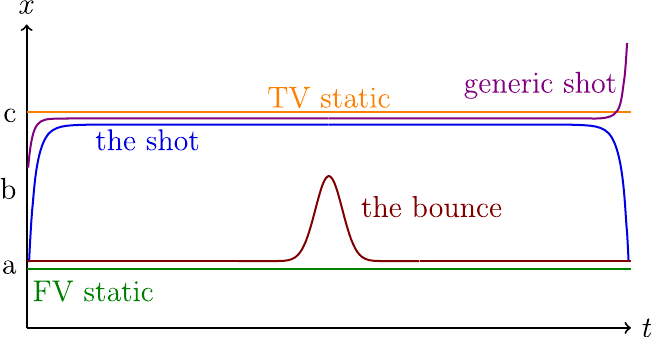
\includegraphics[scale=0.375]{FIGURAS/soluciones}
	\caption{Trayectorias clásicas para el decaimiento del falso vacío.}
	\label{fig:soluciones}
\end{figure}


%Notamos rápidamente que tenemos una primera trayectoria clásica en la que la partícula permanece en el falso vacío todo el tiempo. Llamaremos a esta solución  
%es la solución trivial de \eqref{eq:mov_ec} que cumple  \eqref{eq:cond_frontera}.

Analizando el potencial invertido de la figura 

\begin{figure}[h]
	\centering
	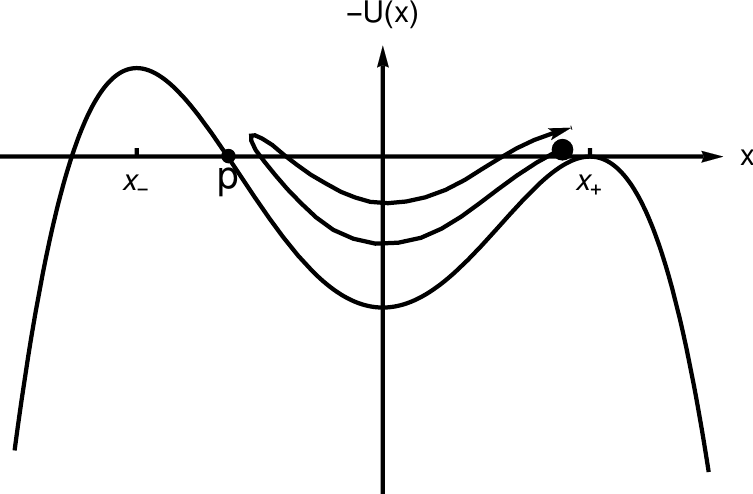
\includegraphics[scale = 0.3]{FIGURAS/potencial_invertido}
	\caption{Potencial invertido \cite{Ai:2019dqr}.}
	\label{fig:potencial_invertido}
\end{figure}


\section{Modo zero}

\section{Modo negativo}

Normalmente, la amplitud no contiene una parte imaginaria. Sin embargo, por continuación analítica adquiere una. 

\section{Contribución multibounce}
\chapter[Decaimiento del falso vacío en la TCC]{Decaimiento del falso vacío en la Teoría Cuántica de Campos}

%\section{Soluciones a la ecuación de movimiento}

\section{Tasa de decaimiento del falso vacío por unidad de volumen
	%en la Teoría Cuántica de Campos
}

Consideremos el campo escalar $\phi\qty(x)$ cuya acción $S\qty[\phi\qty(x)]$ está dada por %\footnote{$x=\qty(t, x, y, z)$ es el cuadrivector posición.} 
\begin{equation} \label{eq:accion_qft}
S\qty[\phi\qty(x)] = \int \dd[4]{x} \qty[\frac{1}{2}\qty(\pdv{\phi}{t})^2 - \frac{1}{2}\qty(\grad{\phi})^2 - U\qty(\phi) ]
\end{equation}
donde el potencial 
%\footnote{$U\qty(\phi)$ es la densidad de potencial pero por comodidad no usaremos esta denominación.} 
$U\qty(\phi)$ está dado en la figura \ref{fig:potencial_qft}. Cuenta con dos mínimos $\phi_-$ y $\phi_+$, de los cuales este último es un falso vacío por lo que, al igual que en la Mecánica Cuántica, 
%revisar terminos: "se encuentre" o "tenga una configuracion"
esperamos que, si la configuración inicial del campo es $\phi_+$, 
exista una cierta probabilidad de que
pueda decaer a $\phi_-$ por tunelamiento. Resulta conveniente añadirle una constante 
%a $U\qty(\phi)$ 
de tal manera que $U\qty(\phi_+) = 0$ y la energía del campo en el falso vacío sea finita \cite{andreassen2017precision}. 
\begin{figure}[t]
	\centering
	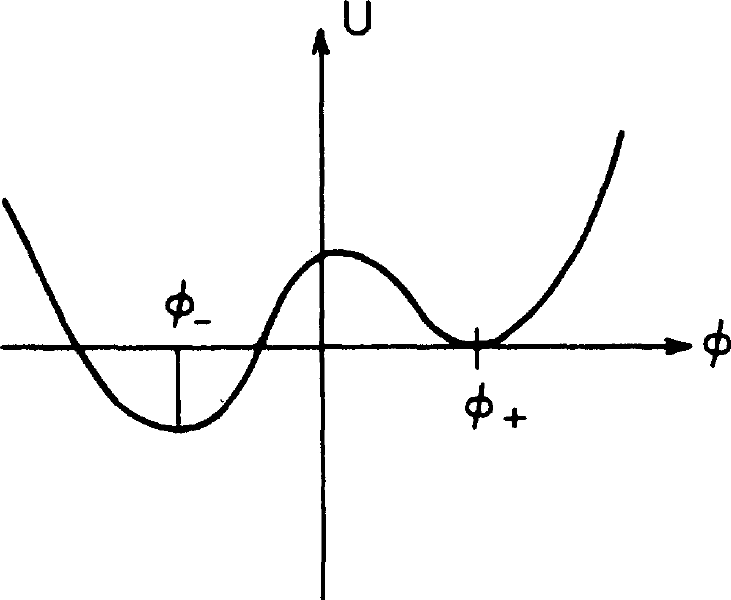
\includegraphics[scale=0.25]{FIGURAS/potencial_qft}
	\caption{Potencial en el que se encuentra el campo escalar dado por la acción \eqref{eq:accion_qft}. Notamos que cuenta con un falso vacío en $\phi_+$ \cite{callan1977fate}.}
	\label{fig:potencial_qft}
\end{figure}

A pesar de esto, la energía del campo en el verdadero vacío es infinita debido a que $U\qty(\phi_-)$ es distinto de cero e integramos sobre todo el espacio \cite{paranjape2017theory}. De la misma manera, la barrera de potencial a través de la cual se debe dar el tunelamiento, también es infinita, por lo que el decaimiento del falso vacío solo puede darse en ciertas regiones del espacio. 
%Como esta es arbitraria, la tasa de decaimiento es proporcional al volumen y por lo tanto, infinita \cite{weinberg2012classical}.  
%añadir algo sobre que la diferencia de energia respecto al falso vacio es finita
Es por esto que la cantidad físicamente relevante a calcular es la tasa de decaimiento del falso vacío por unidad de volumen $\Gamma/V$ \cite{weinberg2012classical} de la forma
\begin{equation} \label{eq:gamma_volumen_WKB}
\frac{\Gamma}{V} = Ae^{-B/\hbar}\qty(1 + \order{\hbar}),
\end{equation}
% serán discutidas más adelante. 
donde $A$ y $B$ son coeficientes a determinar mediante la extensión del formalismo desarrollado en el capítulo anterior a la Teoría Cuántica de Campos del campo escalar. 



\section{Bounces en la Teoría Cuántica de Campos}

%Habiendo desarrollado el formalismo 
Si bien al momento de calcular $\Gamma/V$ haremos uso del formalismo desarrollado en el capítulo anterior,
%adaptado, mediante analogía con lo estudiado 
previamente debemos plantear el problema clásico correspondiente con sus respectivas condiciones de frontera y encontrar 
%las configuraciones clásicas  
las configuraciones clásicas del campo que no son más que las soluciones a la ecuación de movimiento.  

Al aplicar el cambio de variable a tiempo imaginario \eqref{eq:tiempo_im} en la acción \eqref{eq:accion_qft} tenemos que $\phi = \phi\qty(\tau, \vb{x})$ \footnote{A partir de ahora trabajaremos exclusivamente en tiempo euclideano. 
%en lo que resta de la sección 
%por lo que  omitiremos la dependencia funcional de $\phi = \phi\qty(\tau, \vb{x})$ en la medida de lo posible.
} 
y su acción euclideana $S_E\qty[\phi\qty(\tau, \vb{x})]$ está dada por
\begin{equation}
S_E\qty[\phi\qty(\tau, \vb{x})] = \int \dd{\tau} \dd[3]{x} \qty[\frac{1}{2}\qty(\pdv{\phi}{\tau})^2 + \frac{1}{2}\qty(\grad{\phi})^2 + U\qty(\phi)]
\end{equation}
junto con la ecuación de movimiento correspondiente
\begin{equation} \label{eq:eom_phi}
\qty(\pdv[2]{\tau} + \grad{}^2)\phi = U'\qty(\phi),
\end{equation}
donde la prima indica la derivada respecto a $\phi\qty(\tau, \vb{x})$. 

Como estamos interesados en las configuraciones clásicas,
%puesto que este es un punto estacionario de la acción. Inicialmente el campo se encuentra en el falso vacío
debemos establecer las condiciones de frontera adecuadas para la ecuación de movimiento \eqref{eq:eom_phi}. Sabemos que la solución no trivial relevante en el decaimiento del falso vacío es el bounce. Es decir, buscamos una configuración que parta de $\phi_+$, atraviese la barrera hasta llegar al punto de retorno y finalmente, regrese de vuelta a $\phi_+$.  De esta manera, podemos trasladar todas las consideraciones estudiadas anteriormente en la Mecánica Cuántica a la Teoría Cuántica de Campos del campo escalar. 

Tenemos entonces la primera condición de frontera 
%Bajo las mismas consideraciones 
\begin{equation} \label{eq:cond_frontera_qft1}
\lim_{\tau \rightarrow \pm\infty} \phi\qty(\tau, \vb{x}) = \phi_+,
\end{equation}
%donde hemos establecido $\tau_i = -\infty$ y $\tau_f = +\infty$ puesto que esperamos obtener el bounce en el límite . %puesto que este es el límite en el que estamos interesados. 
%que nos asegura que tanto la configuración inicial como final del campo es el falso vacío. 
la cual establece que el
%la configuración del 
campo permanece en el falso vacío durante un tiempo euclideano lo suficientemente largo antes y después de atravesar la barrera. Cabe resaltar que este comportamiento simétrico es debido al hecho de que la acción es invariante ante una inversión temporal. Como hemos establecido la condición de frontera \eqref{eq:cond_frontera_qft1} para un tiempo euclideano que tiende al infinito, 
%por conveniencia, 
podemos fijar el instante en el que el campo llega al punto de retorno en $\tau = 0$,
\begin{equation} \label{eq:cond_frontera_qft2}
\pdv{\phi}{\tau}\qty(0, \vb{x}) = 0,
\end{equation}
%Podemos hacer esto debido al límite que estamos considerando.
%\begin{equation}
%	\mathcal{E} = \frac{1}{2}\qty(\pdv{\phi}{\tau})^2 - \frac{1}{2}\qty(\grad{\phi})^2 - U\qty(\phi)
%\end{equation}
de tal manera que la energía cinética del campo sea igual a cero una vez que haya cruzado la barrera. 
Por último, la acción del bounce debe ser finita. Caso contrario, el coeficiente $B$ en la ecuación \eqref{eq:gamma_volumen_WKB}, se anularía \cite{lee2005fate}. Como $U\qty(\phi_+) = 0$,
%\begin{equation}
%\mathcal{E} = \frac{1}{2}\qty(\pdv{\phi}{\tau})^2 - \frac{1}{2}\qty(\grad{\phi})^2 - U\qty(\phi)
%\end{equation}
\begin{equation} \label{eq:cond_frontera_qft3}
\lim_{\qty|\vb{x}| \rightarrow \pm\infty} \phi\qty(\tau, \vb{x}) = \phi_+,
\end{equation}
el campo se encuentra en el falso vacío a grandes distancias \cite{Masoumi:2015psa}. %\subsection{Soluciones a la ecuación de movimiento}
%Habiendo establecido las condiciones de frontera

\begin{figure}[t]
	\centering
	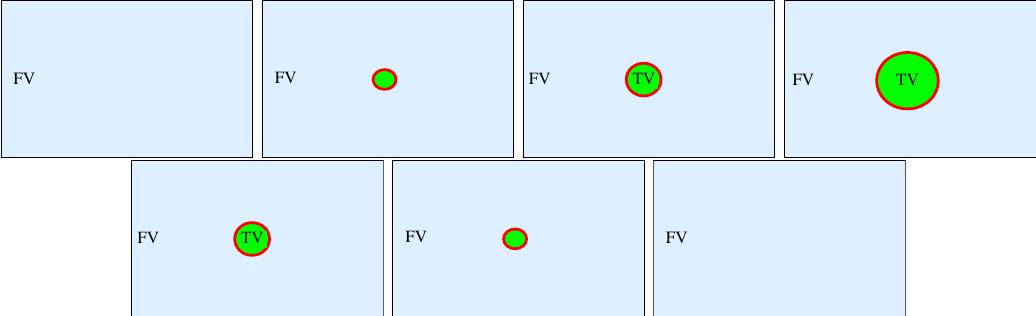
\includegraphics[scale=0.4]{FIGURAS/nucleacion_burbujas}
	\caption{Proceso de nucleación de una burbuja de falso vacío \cite{Masoumi:2015psa}.}
	\label{fig:nucleacionburbujas}
\end{figure}
Analicemos cualitativamente el comportamiento del bounce. Inicialmente, el campo se encuentra en el falso vacío a lo largo de todo el espacio.
%, tal como se indica en la primera condición de frontera \eqref{eq:cond_frontera_qft1}. 
En un cierto instante de tiempo euclideano y en una cierta región del espacio, el campo decae al verdadero vacío mientras que lejos de este, permanece inafectado. Es decir, aparece una burbuja de verdadero vacío 
%tal como se puede ver en la figura , %insertar figura
que empieza a crecer hasta alcanzar su tamaño máximo en $\tau = 0$, a partir del cual se encoge hasta desaparecer, regresando finalmente a la configuración inicial. Todo este proceso se ilustra en la figura \eqref{fig:nucleacionburbujas}
%Este proceso 
y es análogo al proceso de nucleación de burbujas de vapor en la Mecánica Estadística \cite{coleman1977fate}, razón por la cual al bounce también se le denomina burbuja. 

Como es de esperarse, la ecuación de movimiento \eqref{eq:eom_phi} cuenta con una solución trivial que, de acuerdo con la condición de frontera en \eqref{eq:cond_frontera_qft1}, está dada por
\begin{equation} \label{eq:phi_trivial}
	\phi_{\text{FV}}\qty(\tau, \vb{x}) = \phi_+.
\end{equation}
%Tal como se expuso en el párrafo anterior, las soluciones no triviales 

Las ecuación de movimiento \eqref{eq:eom_phi}, las condiciones de frontera \eqref{eq:cond_frontera_qft1} y \eqref{eq:cond_frontera_qft3} y la interpretación del bounce como una burbuja de verdadero vacío, sugieren asumir que este último cuenta con una simetría $O\qty(4)$, es decir, es invariante ante rotaciones del espaciotiempo euclideano o esféricamente simétrico \cite{weinberg2012classical}. Para una gran cantidad de potenciales, esto siempre es posible 
%encontrar un bounce de esta forma 
\cite{coleman1978action}. 

Introduzcamos la distancia euclideana
\begin{equation}
	\rho^2 \equiv \tau^2 + \vb{x}^2
\end{equation}
de tal manera que, de acuerdo con lo establecido anteriormente,  $\phi = \phi\qty(\rho)$. 
%mientras que \eqref{eq:cond_frontera_qft2},
%\begin{equation}
%\eval{\pdv{\phi\qty(\rho)}{\tau}}_{\tau = 0} = 0.
%\end{equation}
%Como $\rho = \rho(\vb{x}, \tau)$, tenemos que
%\begin{equation}
%\pdv{\phi\qty(\rho)}{\tau} = \dv{\phi}{\rho}\pdv{\rho}{\tau}.
%\end{equation}
%
%\begin{align}
%	2\rho \pdv{\rho}{\tau} &= 2\tau \\
%	\pdv{\rho}{\tau} &= \frac{\tau}{\rho}
%\end{align}
%\begin{equation}
%\eval{\dv{\phi\qty(\rho)}{\tau}}_{\rho = 0} = 0
%\end{equation}
%\begin{equation}
%\eval{\dv{\phi}{\rho}}_{\rho = 0} = 0
%\end{equation}
Resulta conveniente renombrar $\tau = x_4$ de tal manera que 
\begin{equation} \label{eq:rho_xi}
	\rho^2 = \sum_{i = 1}^{4} x_i^2.
\end{equation}
%donde $\vb{x} = \qty(x, y, z) = \qty(x_1, x_2, x_3)$. 
De acuerdo con esta notación, la ecuación de movimiento \eqref{eq:eom_phi} está dada por
\begin{equation} \label{eq:eom_xi}
\sum_{i = 1}^{4} \pdv[2]{\phi\qty(\rho)}{x_i} = U'\qty(\phi).
\end{equation}
Escrita de esa manera obtendremos 
%fácilmente la ecuación de movimiento para 
la correspondiente a $\phi\qty(\rho)$. 
%nos facilitará el cambio de variable. 
Haciendo uso de la regla de la cadena, 
\begin{equation} \label{eq:dv_phi_rho}
	\pdv{\phi\qty(\rho)}{x_i} = \dv{\phi}{\rho}\pdv{\rho}{x_i}.
%	&= \frac{x_i}{\rho}\dv{\phi}{\rho}.
\end{equation}
Derivando \eqref{eq:rho_xi} respecto a $x_i$,
\begin{align}
2\rho \pdv{\rho}{x_i} &= 2x_i \\ \label{eq:dv_rho_xi}
\pdv{\rho}{x_i} &= \frac{x_i}{\rho}
\end{align}
y reemplazando esta última
%\eqref{eq:dv_rho_xi} 
en \eqref{eq:dv_phi_rho}, 
\begin{equation} \label{eq:dv_phi_rho2}
\pdv{\phi\qty(\rho)}{x_i} = \frac{x_i}{\rho}\dv{\phi}{\rho}.
\end{equation}
Derivando la ecuación anterior
%\eqref{eq:dv_phi_rho2} 
respecto a $x_i$ y usando nuevamente \eqref{eq:dv_rho_xi},
\begin{align}
	\pdv[2]{\phi\qty(\rho)}{x_i} &= \frac{x_i}{\rho}\dv[2]{\phi}{\rho}\pdv{\rho}{x_i} + \qty(\frac{1}{\rho} - \frac{x_i}{\rho^2}\pdv{\rho}{x_i})\dv{\phi}{\rho} \\
	&= \frac{x_i^2}{\rho^2}\dv[2]{\phi}{\rho} + \frac{1}{\rho}\qty(1 - \frac{x_i^2}{\rho^2})\dv{\phi}{\rho}. 
\end{align}
Por último, sumamos las derivadas,
\begin{align}
\sum_{i = 1}^{4} \pdv[2]{\phi\qty(\rho)}{x_i} &=  \frac{\sum_{i = 1}^{4} x_i^2}{\rho^2}\dv[2]{\phi}{\rho} + \frac{1}{\rho}\qty(4 - \frac{\sum_{i = 1}^{4} x_i^2}{\rho^2})\dv{\phi}{\rho}, 
\end{align}
y simplificamos haciendo uso de \eqref{eq:rho_xi} para obtener finalmente la ecuación de movimiento 
%en términos de $\phi\qty(\rho)$
\begin{equation} \label{eq:eom_rho}
	\dv[2]{\phi}{\rho} + \frac{3}{\rho}\dv{\phi}{\rho} = U'\qty(\phi).
\end{equation}

Las condiciones de frontera \eqref{eq:cond_frontera_qft1} y \eqref{eq:cond_frontera_qft3} se reducen a 
\begin{equation} \label{eq:cond_frontera_rho1}
\lim_{\rho \rightarrow \pm\infty} \phi\qty(\rho) = \phi_+.
\end{equation}
Con la finalidad de evitar que las soluciones cuenten con una singularidad en el origen, requerimos que \cite{coleman1977fate}
\begin{equation}
	\eval{\dv{\phi}{\rho}}_0 = 0.
\end{equation}

La ecuación de movimiento \eqref{eq:eom_rho} puede ser interpretada como la ecuación de movimiento de una partícula 

%analisis clasico de la eom
%argumento overshoot-undershoot de la existencia de la solucion

\subsection{Aproximación de la pared delgada}

El campo dentro de la burbuja, en realidad corresponde al punto de retorno y no al verdadero vacío \cite{lee2005fate}. 

\section{Cálculo de la tasa de decaimiento del falso vacío por unidad de volumen}

Habiendo obtenido las configuraciones clásicas relevantes en el decaimiento del falso vacío, procedemos al cálculo de la tasa de decaimiento del falso vacío por unidad de volumen $\Gamma/V$. Siguiendo el formalismo de Coleman y Callan, partimos de la amplitud de transición 
\begin{equation}
I = \bra{\phi_f}e^{-HT/\hbar}\ket{\phi_i} = \int \mathcal{D}\phi \, e^{-S_E\qty[\phi\qty(\vb{x},\tau)]/\hbar}.
\end{equation}
De acuerdo con la condición de frontera \eqref{eq:cond_frontera_qft1}, $\phi_i = \phi_f = \phi_+$.

Las burbujas de falso vacío pueden aparecer en cualquier región del espacio, es decir, son invariantes ante translaciones espaciales \cite{coleman1977fate}. 

Es posible demostrar que el modo negativo es único para todos los casos de interés \cite{coleman1977fate, coleman1988quantum}

\section{El destino del falso vacío}

\subsection{Implicaciones cosmológicas}

\subsection{Aplicaciones}
\chapter{Conclusiones}

Si bien hemos podido calcular la tasa de decaimiento $\Gamma$ para el decaimiento del falso vacío, quedan varias preguntas conceptuales que no podrán ser abordadas en este trabajo de investigación y que tampoco se discuten a profundidad en la literatura consultada. Por ejemplo, la hermiticidad 

Por último, pero no por eso menos importante, el presente trabajo de investigación representa una pequeña contribución a la literatura en español sobre el decaimiento del falso vacío y espero puede ser utilizada como referencia en investigaciones futuras. 

\printbibliography
\addcontentsline{toc}{chapter}{Bibliografía}

\end{document}